\section{評価実験}
\label{評価実験}

本章では\ref{対話システムの構築}章で説明した対話システムについて,大阪府吹田市にある大型複合施設EXPOCITY内にあるショッピングモール「らぽーとEXPOCITY」で行われた対話ロボットコンペティション\footnote{https://sites.google.com/view/crobotcompetition}に参加し,評価実験を行う.

\subsection{実験設定}

\subsubsection{旅行代理店対話タスク}
対話ロボットコンペティションでは,旅行代理店における対話タスクとして,カウンターセールス役となったロボットが,対話を通してお客様役である対話者の要望に応える.体験者は図\label{6place}に示す通り,「日本民家集落博物館」,「茨木市立川端康成文学館」,「総持寺」,「日本民家集落博物館」,「箕面大滝」,「明治なるほどファクトリー大阪」の6箇所の観光地候補から行きたい2箇所決め,そのどちらに行きたいをシステムとの対話を通して決める.
\begin{figure}[th]
    \centering
    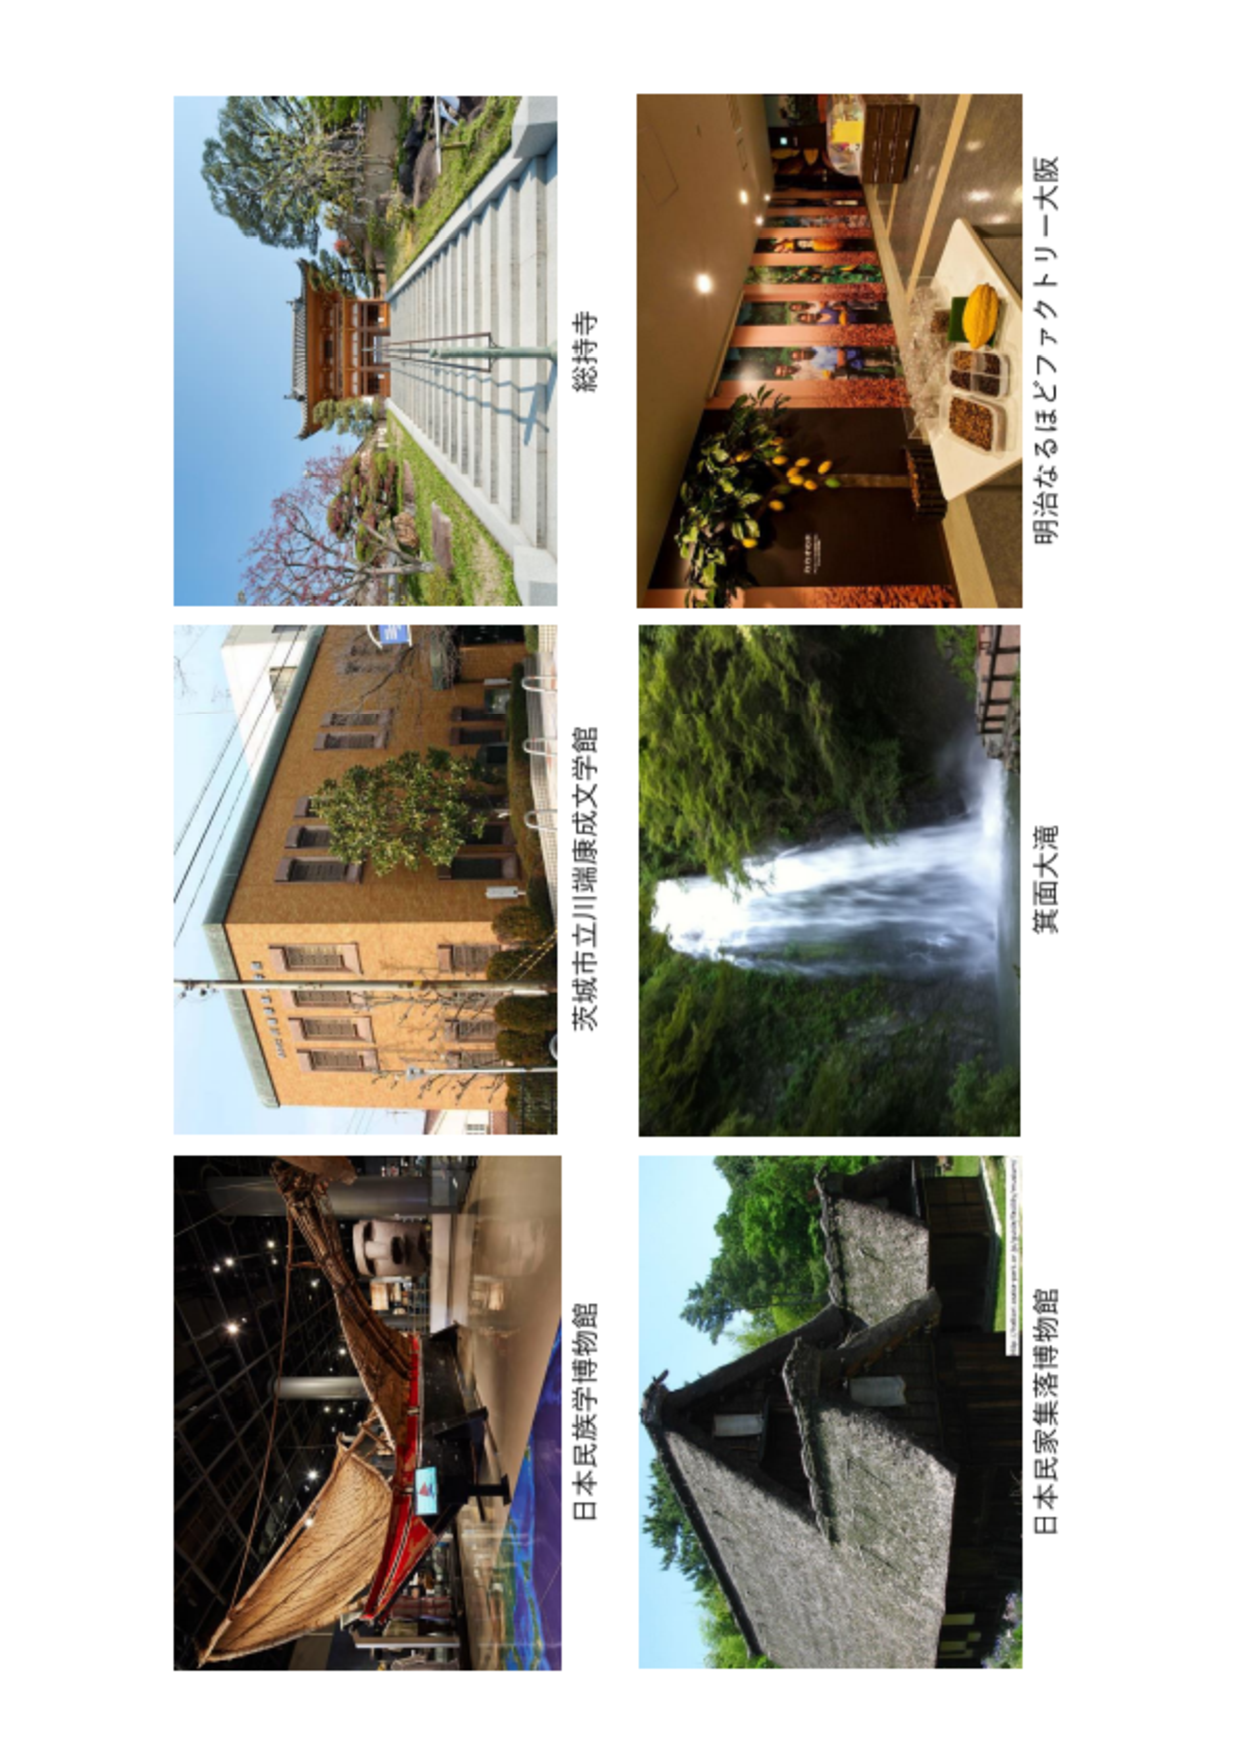
\includegraphics[scale=0.5,angle=270]{pic/6place.pdf}
    \caption{観光地の候補}
    \label{6place}
\end{figure}

\subsubsection{体験やへの事前の指示}
ロボットと対話する体験者は,当日らぽーとEXPOCITYを訪れた買い物客であるため,実際に対話をするにあたり,以下のような事前の指示を行う.

\begin{itemize}
    \item 日本語でロボットと対話して頂きます.
    \item お客様役として振る舞って頂きます.
    \begin{itemize}
        \item Expo Cityに休暇で訪れる予定を持っており,その近辺で1日遊びに行く観光地を決める目的を持っているつもりになって,カウンターセールス役のロボットに相談してください.
        \item 対話を行う前に,近辺の観光地候補の中から行ってみたいと思う観光地を2箇所選んでください.カウンターセールス役のロボットと相談して,体験者自身がお金を払ってでも遊びに行きたいと思える観光地をその2箇所の中から1箇所を決めてください.
        \item 2つの観光地に関する情報をまんべんなく確認して,行きたい観光地を決めてください.
    \end{itemize}
    \item 対話中の注意事項
    \begin{itemize}
    \item カウンターの椅子に座ってから対話を始めてください.
    \item ロボットと相談する時間は最大5分間です.5分経過すると対話を終えて頂きます.5分経過する前に行きたい場所が決まった場合は,カウンター上のタブレットの「行きたい場所を決めた」ボタンにタッチして対話を終えてください.
    \item 相談が終わった後,カウンター上のタブレット上に,ただいまの対話についての質問が表示されますので,それについて回答して頂いた後,行きたい観光地(強いて行きたいならどこか)を選んでください(対話を通して観光地の情報がうまく聞き出せなかった場合などで選ぶのが難しい場合は「選べない」を選択して頂くことも可能です).
    \item 最後に,体験についてのアンケートについてタブレットで回答して頂きます.
    \end{itemize}
\end{itemize}

\subsubsection{レギュレーション}
対話ロボットコンペティションではレギュレーションが定められており,このレギュレーションに従って開発,実装を行なう.
\begin{enumerate}
    \item 対話状況
    \begin{itemize}
        \item 体験者とロボットは1対1で対話する.
        \item カウンターテーブルの大きさ,ロボットと体験者の椅子の位置は固定.
        \item テーブル上に体験者とロボットが同時に見ることができるようにモニタを設置(位置と向きは固定).
    \end{itemize}
    \begin{figure}[th]
        \centering
        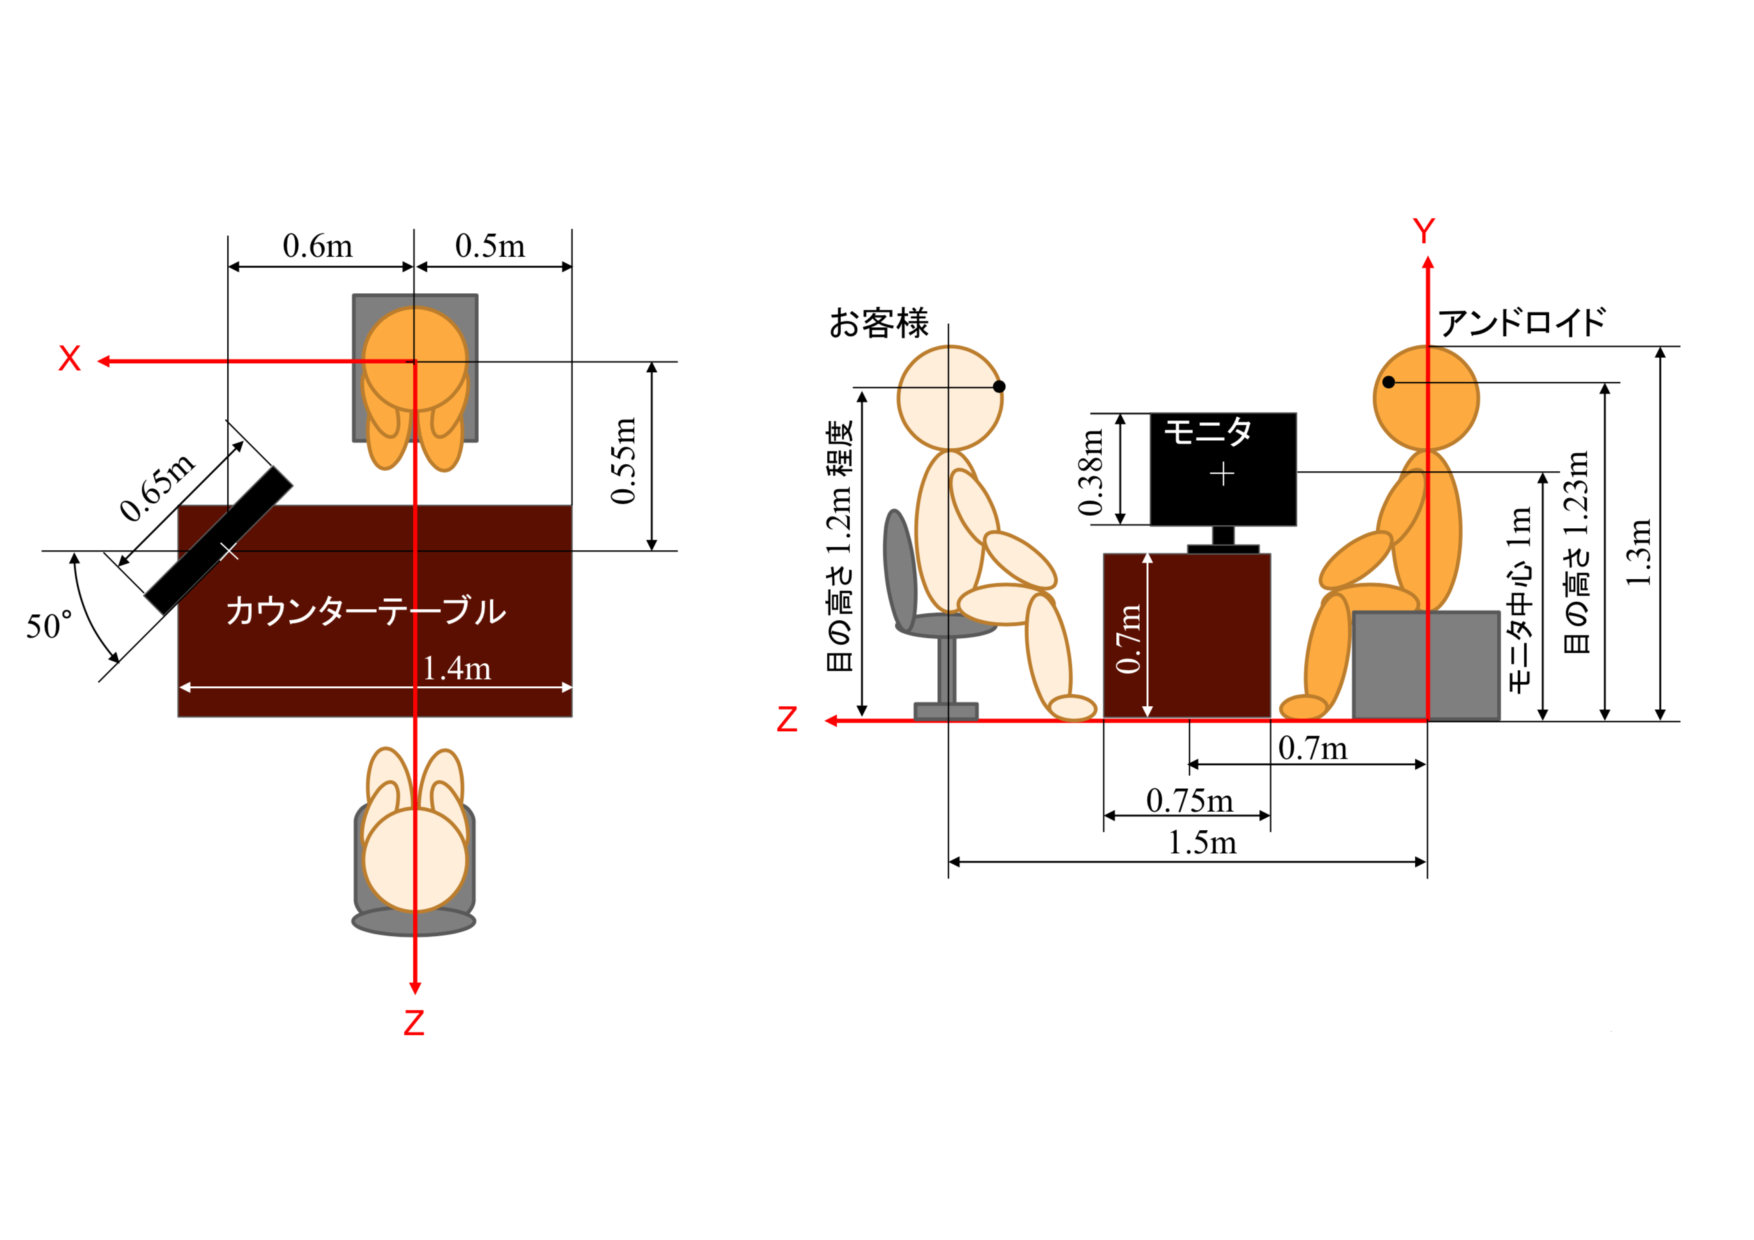
\includegraphics[scale=0.5,angle=270]{pic/robot_location.pdf}
        \caption{体験者とロボットの位置関係}
    \end{figure}
    \item ロボットに行わせてもよいこと
    \begin{itemize}
        \item 任意のタイミングで発話させること.
        \item 任意のタイミングで,視線,表情,頭部,上体等を動かすこと.
        \item 貸与された観光地情報を用いて説明すること.
        \item カウンター上のモニタに表示された観光地の写真について説明すること.
        \item 説明している観光地についての感想や意見を言うこと.ただし,開発指針として,本番で未知の観光地情報が与えられたとしても対応できるようにシステムを開発すること.
    \end{itemize}
    \item ロボットが対話中に使える情報
    \begin{itemize}
        \item 参加登録時に貸与される12箇所の観光地に関する観光案内情報.
        \item マイクとカメラで認識された,体験者の音声,表情,性別,年齢.
        \item モニタの位置(置いてある場所)の情報.
    \end{itemize}
    \item 観光地情報の扱い方
    \begin{itemize}
        \item 観光地情報データベースのレコードをプログラムで自由に操作して利用してよいものとする.
        \item 参加登録時に,本番で使用する観光地情報を渡すが,開発指針として,本番で未知の観光地情報が与えられたとしても対応できるようにシステムを開発すること.
    \end{itemize}
    \item 提案する観光地とお薦めの観光地
    \begin{itemize}
        \item 提案する観光地:対話開始前に,体験者は日本科学未来館近辺の6箇所,あるいはExpo City近辺の6箇所の観光地の中から,行ってみたいと思う観光地を2つ選ぶ.
        \item お薦めの観光地:2箇所の中からランダムに決定.
    \end{itemize}
    \item 対話タスクの開始・終了
    \begin{itemize}
        \item タスク開始前に,体験者から聞き出した2か所の観光地(A,B),その中からランダムに決定したお薦め観光地を参加者のプログラムに入力.
        \item テーブルのモニタ上に,観光地AとBの写真を並べて出力(Aが左,Bが右)モニタへの出力は主催者側で実行
        \item 体験者が椅子に着席した状態で,参加者のプログラムを開始.
        \item 対話開始から5分経過した時点,あるいは体験者がテーブル上のタブレットで観光地を決めたことを知らせてきた時点で,参加者のプログラムに対話終了.命令を入力し,対話タスクを終了.対話開始から5分経過しても対話中である場合は,体験者にタブレットで対話を終えるように伝える(主催者側が用意).
        \item 対話の始まりは,ロボットから話始めても,お客様の話始めを待っても,どちらでもよいとする.
        \item 対話終了後に,体験者にタブレットで観光地を選んでもらう.
    \end{itemize}
    \begin{figure}[th]
        \centering
        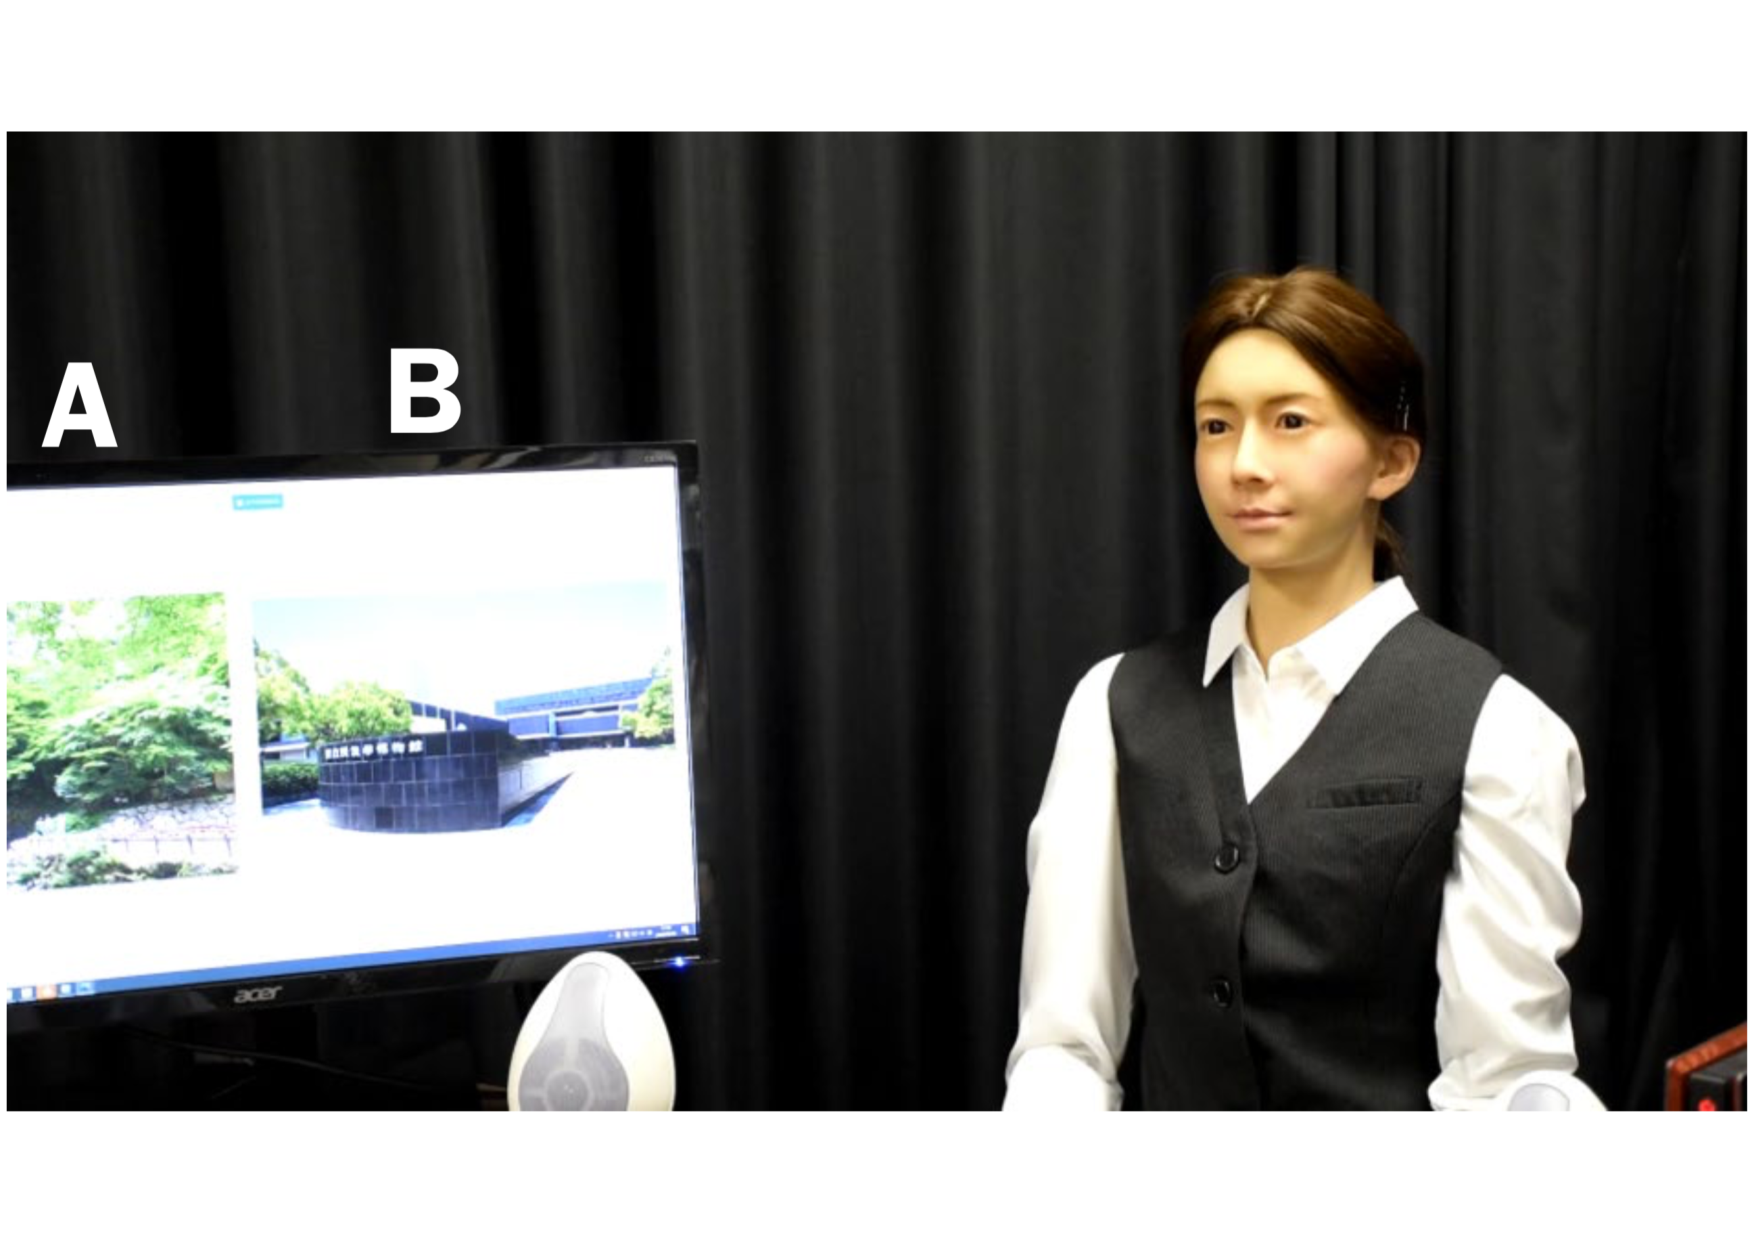
\includegraphics[scale=0.5,angle=270]{pic/AB_location.pdf}
        \caption{観光地の出力}
    \end{figure}
    \item ロボットに行わせてはいけないこと
    \begin{itemize}
        \item 対話以外の方法で,お薦めの観光地を体験者に選んでもらうこと(例:ロボットが,体験者に,お薦めの観光地を選んでもらったら賞品をあげるなどと言う).
    \end{itemize}
\end{enumerate}

\subsection{対話の評価手法}
下記の2つの観点から,システムの総合的な評価を行う.
\begin{itemize}
    \item カウンターセールスとしてお薦めの観光地を選んでもらえたかどうか
    \item 体験者の満足度(対話後のアンケートによる評価)
\end{itemize}
アンケート評価の評価項目は,下記の8つの観点である.1点の「そう思わない」7点の「そう思う」までの7段階で評価を行う.
\subsubsection{対話者の評価手法}
\begin{enumerate}
    \item 満足して遊びに行く観光地を選ぶことができましたか?(選択の満足度)
    \item 観光地の情報を十分に聞くことができましたか?(情報の十分さ)
    \item ロボットとは自然に対話できましたか? (対話の自然さ)
    \item ロボットの対応は適切でしたか?(対話の適切さ)
    \item ロボットとの対話に満足しましたか?(対話の満足度)
    \item ロボットの対応は好ましいものでしたか?(対応の好ましさ)
    \item 観光地を選ぶのにロボットから得られた情報を参考にしましたか?(情報の参考度)
\end{enumerate}

\subsubsection{ビデオ評価の評価手法}
COVID-19の影響で対話者が想定より集まらず,チーム間での対話者の人数にばらつきがあるため,参加チームごと予選会場での対話を記録した映像を用いて,クラウドで追加の印象評価を実施する.評価項目は,下記の8つの観点である.1点の「そう思わない」7点の「そう思う」までの7段階で評価を行う.システムが正常に動かなかった場合などを評価から排除できるよう,各チームが3つの対話映像を選択し,それらを第三者に評価させる.
\begin{itemize}
    \item お客様とロボットの対話を第三者視点でどう思うかお答えください.
    \begin{enumerate}
        \item お客様はロボットから観光地の情報を十分に聞けていましたか?(情報の十分さ(客視点))
        \item お客様はロボットと自然に対話できていましたか?(対話の自然さ(客視点))
        \item お客様はロボットの対応を好ましく思っていましたか?(対応の好ましさ(客視点))
        \item お客様はロボットの対応に満足していましたか?(対応の満足度(客視点))
    \end{enumerate}
    \item あなたがこのロボットと対話したお客様だったらという視点でどう思うかお答えください.
    \begin{enumerate}
        \item あなたはロボットから観光地の情報を十分に聞けたと思いますか?(情報の十分さ(評価者視点))
        \item あなたはロボットと自然に対話できたと思いますか?(対話の自然さ(評価者視点))
        \item あなたはロボットの対応を好ましかったと思いますか?(対応の好ましさ(評価者視点))
        \item あなたはロボットの対応に満足したと思いますか?
        \item ロボットの話を聞いてあなたならどちらの観光地に行きたいと思いましたか?(どちらとも言えない場合は、強いて決めるとしたらどちらかで決めてください)
        \item このロボットは旅行代理店で実際にサービスできると思いますか?
    \end{enumerate}
\end{itemize}

\subsection{実験結果}
2021年8月23日,9月4日の二日間にかけて,10代から50代の男女21人によって評価を行なった.コンペティション全体として,大学8,高専1,企業2の11チームがコンペティションに参加し,それぞれ別日に同様の評価を行う.ビデオ評価は参加11チームのシステムと,実行委員の用意したベースラインを含めた12のシステムについて評価を行う・

\subsection{対話結果}
21

\subsection{アンケート評価の結果}
体験者21人のアンケート結果から表\ref{result_taiken}のような評価が得られ,ビデオ評価者50人のアンケート結果から表\ref{result_video}から以下のような評価が得られた.

\begin{table}[hbtp]
    \caption{体験者によるアンケート結果}
    \label{result_taiken}
    \centering
    \begin{tabular}{l|l|l|l|l|l|l|l}
    \hline
          & 選択の満足度 & 情報の十分さ & 対話の自然さ & 対話の適切さ & 対話の満足度 & 対応の好ましさ & 情報の参考度 \\ \hline
    評価の平均 & 4.05   & 4.10   & 3.14   & 3.62   & 3.86   & 4.00    & 4.24   \\ \hline
    順位    & 12     & 12     & 9      & 10     & 8      & 8       & 12     \\ \hline
    \end{tabular}
\end{table}

\begin{table}[hbtp]
    \caption{ビデオ評価によるアンケート結果}
    \label{result_video}
    \centering
    \begin{tabular}{llllll}
    \hline
    客観視点                    &                             &                             &                              &                             &      \\ \hline
    \multicolumn{1}{l|}{}   & \multicolumn{1}{l|}{情報の十分さ} & \multicolumn{1}{l|}{対話の自然さ} & \multicolumn{1}{l|}{対話の適切さ}  & 対話の満足度                      &      \\ \hline
    \multicolumn{1}{l|}{評価} & \multicolumn{1}{l|}{4.10}   & \multicolumn{1}{l|}{3.76}   & \multicolumn{1}{l|}{3.62}    & 3.86                        &      \\ \hline
    \multicolumn{1}{l|}{順位} & \multicolumn{1}{l|}{11}     & \multicolumn{1}{l|}{9}      & \multicolumn{1}{l|}{10}      & 8                           &      \\ \hline
    評価者視点                   &                             &                             &                              &                             &      \\ \hline
    \multicolumn{1}{l|}{}   & \multicolumn{1}{l|}{情報の十分さ} & \multicolumn{1}{l|}{対話の自然さ} & \multicolumn{1}{l|}{対話の好ましさ} & \multicolumn{1}{l|}{対話の満足度} & 実用性  \\ \hline
    \multicolumn{1}{l|}{評価} & \multicolumn{1}{l|}{3.96}   & \multicolumn{1}{l|}{3.90}   & \multicolumn{1}{l|}{3.81}    & \multicolumn{1}{l|}{3.51}   & 3.74 \\ \hline
    \multicolumn{1}{l|}{順位} & \multicolumn{1}{l|}{10}     & \multicolumn{1}{l|}{11}     & \multicolumn{1}{l|}{11}      & \multicolumn{1}{l|}{11}     & 11   \\ \hline
    \end{tabular}
\end{table}
